\begin{name}
	{\tenchude}
	{\tendethi}
	{\tentruong}
	{\thoigian}
\end{name}
\Opensolutionfile{ans}[ans/ans-De08HT]
%%%=========Cau_1=========%%%
% \begin{ex}%[2D2B5-2]
% 	Tập nghiệm của phương trình $2^{x^2-x-4}=\dfrac{1}{16}$ là
% 	\choice
% 	{$\varnothing$}
% 	{$\left\{2;4\right\}$}
% 	{$\left\{-2;2\right\}$}
% 	{\True$\left\{0;1\right\}$}
% %	{\True $\left\{0;1\right\}$}
% 	\loigiai{Ta có $ 2^{x^2-x-4}=\dfrac{1}{16}\Leftrightarrow{2^{x^2-x-4}}=2^{-4}\Leftrightarrow x^2-x-4=-4\Leftrightarrow x^2-x=0\Leftrightarrow \left[\begin{aligned}
% 	& x=0 \\
% 	& x=1.
% 	\end{aligned}\right.$\\ 
% 	Vậy tập nghiệm của phương trình là $\left\{0;1\right\}$. 
% 	}
% \end{ex}
% %%%=========HetCau_1=========%%%
% %%%=========Cau_2=========%%%
% \begin{ex}%[2D3B2-1]
% 	Cho $\displaystyle\int\limits_{-2}^2f(x)\mathrm{\,d}x=1$, $\displaystyle\int\limits_{-2}^4f(x)\mathrm{\,d}x=-4$. Tính $I=\displaystyle\int\limits_2^4f(x)\mathrm{\,d}x$.\\
% 	\choice
% 	{$I=5$}
% 	{\True $I=-5$}
% 	{$I=-3$}
% 	{$I=3$}
% 	\loigiai{Ta có $\displaystyle\int\limits_{-2}^4f(x)\mathrm{\,d}x=\displaystyle\int\limits_{-2}^2f(x)\mathrm{\,d}x+\displaystyle\int\limits_2^4f(x)\mathrm{\,d}x\Rightarrow \displaystyle\int\limits_2^4f(x)\mathrm{\,d}x=-4-1=-5$.
% 	}
% \end{ex}
% %%%=========HetCau_2=========%%%
% %%%=========Cau_3=========%%%
% \begin{ex}%[2H2Y1-2]
% 	Tính diện tích xung quanh $S$ của khối trụ có bán kính đáy $r=4$ và chiều cao $ h=3 $.
% 	\choice
% 	{$ S=12\pi $}
% 	{$ S=48\pi $}
% 	{\True $ S=24\pi $}
% 	{$ S=96\pi $}
% 	\loigiai{Diện tích xung quanh $ S $ của khối trụ là $ S=2\pi rh=2\pi\cdot4\cdot3=24\pi $ (đvtt).
% 	}
% \end{ex}
% %%%=========HetCau_3=========%%%
% %%%=========Cau_4=========%%%
% \begin{ex}%[2H3Y1-1]
% 	Trong KG $Oxyz$, cho điểm $ M $ thỏa mãn hệ thức $ \overrightarrow{OM}=2\overrightarrow{i}+\overrightarrow{j} $. Tọa độ của điểm $ M $ là
% 	\choice
% 	{\True $ M\left(2;1; 0\right) $}
% 	{$ M\left(2;0;1\right) $}
% 	{$ M\left(0; 2;1\right) $}
% 	{$ M\left(1; 2; 0\right) $}
% 	\loigiai{$ \overrightarrow{OM}=2\overrightarrow{i}+\overrightarrow{j}=2\overrightarrow{i}+\overrightarrow{j}+0\cdot\overrightarrow{k}\Leftrightarrow M\left(2; 1; 0\right) $.
% 	}
% \end{ex}
% %%%=========HetCau_4=========%%%
% %%%=========Cau_5=========%%%
% \begin{ex}%[1D3B3-2]
% 	Cho cấp số cộng $ \left(u_n\right) $ biết $ u_n=2-3n $. Công sai $ d $ của cấp số cộng là
% 	\choice
% 	{$ d=3 $}
% 	{$ d=2 $}
% 	{\True $ d=-3 $}
% 	{$ d=-2 $}
% 	\loigiai{Ta có $ u_{n+1}-u_n=2-3\left(n+1\right)-\left(2-3n\right)=-3, \forall n\in{\mathbb{N}^{*}} $.\\
% 	Vậy cấp số cộng $ \left(u_n\right) $ có công sai $ d=-3 $.
% 	}
% \end{ex}
% %%%=========HetCau_5=========%%%
% %%%=========Cau_6=========%%%
% \begin{ex}%[2H2Y2-1]
% 	Trong không gian với hệ tọa độ $ Oxyz$, cho mặt cầu $ (S)\colon \left(x+1\right)^2+\left(y-2\right)^2+\left(z-1\right)^2=9$. Tìm tọa độ tâm $ I $ và tính bán kính $ R $ của $ (S)$. 
% 	\choice
% 	{\True $ I\left(-1;2;1\right) $ và $ R=3 $}
% 	{$ I\left(1;-2;-1\right) $ và $ R=3 $}
% 	{$ I\left(-1;2;1\right) $ và $ R=9 $}
% 	{$ I\left(1;-2;-1\right) $ và $ R=9 $}
% 	\loigiai{Ta có mặt cầu $ (S) $ có tâm $ I\left(-1;2;1\right) $, bán kính $ R=3 $.
% 	}
% \end{ex}
% %%%=========HetCau_6=========%%%
% %%%=========Cau_7=========%%%
% \begin{ex}%[2D2B1-2]
% 	Cho $ a $ là một số dương, biểu thức $ a^{\tfrac{2}{3}}\sqrt{a} $ viết dưới dạng lũy thừa với số mũ hữu tỉ là
% 	\choice
% 	{$ a^2 $}
% 	{\True $ a^{\tfrac{7}{6}} $}
% 	{$ a^3 $}
% 	{$ a^{\tfrac{1}{6}} $}
% 	\loigiai{Ta có $ a^{\tfrac{2}{3}}\sqrt{a}=a^{\tfrac{2}{3}}\cdot a^{\tfrac{1}{2}} $ $ =a^{\tfrac{2}{3}+\tfrac{1}{2}} $ $ =a^{\tfrac{7}{6}} $.
% 	}
% \end{ex}
% %%%=========HetCau_7=========%%%
% %%%=========Cau_8=========%%%
% \begin{ex}%[2D1B1-2]
% 	\immini{
% 	Cho hàm số $ f(x) $ liên tục trên $ \mathbb{R} $ và có đồ thị như hình vẽ bên. Khẳng định nào sau đây là đúng?
% 	\choice
% 	{\True Hàm số đồng biến trên $ \left(-1;0\right) $ và $ \left(1;+\infty\right) $}
% 	{Hàm số đồng biến trên $ \left(-1;0\right)\cup \left(1;+\infty\right) $}
% 	{Hàm số đồng biến trên $ \left(-\infty;-1\right)\cup \left(1;+\infty\right) $}
% 	{Hàm số đồng biến trên $ \left(-\infty;0\right) $ và $ \left(0;+\infty\right) $}
% 	}{%
% 	\begin{tikzpicture}[scale=0.9, line join = round, line cap = round,>=stealth]
% 	\tikzset{label style/.style={font=\footnotesize}}
% 	\draw[->] (-2,0) --(0,0) node[below right]{$ O $} --(3,0)node[below]{$ x $};
% 	\draw[->](0,-1)--(0,3)node[right]{$ y $};
% 	\draw[domain=-1.65:1.65,smooth=300]
% 	plot(\x,{(\x)^(4)-2*(\x)^(2)+1});
% 	\draw[fill=black](-1,0)circle(1pt)node[below]{$ -1 $} (0,1)circle(1pt)node[above right]{$ 1 $} (1,0)circle(1pt)node[below]{$ 1 $};	
% 	\end{tikzpicture}
% }
% 	\loigiai{Hàm số đồng biến trên $ \left(-1;0\right) $ và $ \left(1;+\infty\right) $.
% 	}
% \end{ex}
% %%%=========HetCau_8=========%%%
% %%%=========Cau_9=========%%%
% \begin{ex}%[2D1B5-1]
% 	\immini{
% 	Đường cong trong hình vẽ bên là đồ thị của hàm số nào dưới đây?
% 	\choice
% 	{ $ y=-x^3+3x^2+1 $}
% 	{$ y=x^3-3x-1 $}
% 	{\True $ y=x^3-3x+1 $}
% 	{$ y=-x^3-3x^2-1 $}
% 	}{%
% 	\begin{tikzpicture}[scale=0.9, line join = round, line cap = round,>=stealth]
% 	\tikzset{label style/.style={font=\footnotesize}}
% 	\coordinate (1)at(1,0);
% 	\coordinate (-1)at(0,-1);
% 	\coordinate (-1')at(-1,0);
% 	\coordinate (1')at(0,1);
% 	\coordinate (3)at(0,3);
% 	\draw[->] (-2.5,0) --(3,0)node[below]{$ x $};
% 	\draw[->](0,-2)--(0,4)node[right]{$ y $};
% 	\draw[domain=-2.1:2.08,smooth=300]
% 	plot(\x,{(\x)^(3)-3*(\x)^(1)+1});
% 	\draw[fill=black](1)circle(1pt)node[above]{$ 1 $} (-1)circle(1pt)node[left]{$ -1 $} (-1')circle(1pt)node[below]{$ -1 $} (1')circle(1pt)node[right]{$ 1 $} (3)circle(1pt)node[right]{$ 3 $};
% 	\draw[dashed](-1,0)--(-1,3)--(0,3) (1,0)--(1,-1)--(0,-1);	
% 	\end{tikzpicture}
% }
% 	\loigiai{Chỉ có đồ thị hàm số $ y=x^3-3x+1 $ đi qua các điểm $ \left(0;1\right) $
% 	và $ \left(1;-1\right) $.
% 	}
% \end{ex}
% %%%=========HetCau_9=========%%%
% %%%=========Cau_10=========%%%
% \begin{ex}%[1D2B2-2]
% 	Từ một nhóm có $ 10 $ học sinh nam và $ 8 $ học sinh nữ, có bao nhiêu cách chọn ra $ 5 $ học sinh trong đó có $ 3 $ học sinh nam và $ 2 $ học sinh nữ?
% 	\choice
% 	{$ \mathrm{C}_{10}^3+\mathrm{C}_8^2 $}
% 	{\True $ \mathrm{C}_{10}^3\cdot \mathrm{C}_8^2 $}
% 	{$ \mathrm{A}_{10}^3\cdot\mathrm{A}_8^2 $}
% 	{$ \mathrm{A}_{10}^3+\mathrm{A}_8^2 $}
% 	\loigiai{Chọn ra $ 3 $ học sinh nam trong $ 10 $ học sinh nam có $ \mathrm{C}_{10}^3 $ cách chọn.\\
% 	Chọn ra $ 2 $ học sinh nữ trong $ 8 $ học sinh nữ có $ \mathrm{C}_8^2 $ cách chọn.\\
% 	Áp dụng quy tắc nhân ta có số cách chọn ra $ 5 $ học sinh trong đó có $ 3 $ học sinh nam và $ 2 $ học sinh nữ là $ \mathrm{C}_{10}^3\cdot \mathrm{C}_8^2 $.
% 	}
% \end{ex}
% %%%=========HetCau_10=========%%%
% %%%=========Cau_11=========%%%
% \begin{ex}%[2D1B4-1]
% 	Đường tiệm cận ngang, đường tiệm cận đứng của đồ thị hàm số $ y=\dfrac{2x-1}{x-2} $ lần lượt có phương trình là
% 	\choice
% 	{$ y=2, x=\dfrac{1}{2} $}
% 	{$ x=2, y=2 $}
% 	{\True $ y=2, x=2 $}
% 	{$ y=2, x=-2 $}
% 	\loigiai{Ta có:\\
% 	$ \lim\limits_{x\to +\infty}\dfrac{2x-1}{x-2}=2; \lim\limits_{x\to -\infty}\dfrac{2x-1}{x-2}=2 $, suy ra đường thẳng $ y=2 $ là đường tiệm cận ngang.\\
% 	$ \lim\limits_{x\to{2^{+}}}\dfrac{2x-1}{x-2}=+\infty; \lim\limits_{x\to{2^{-}}}\dfrac{2x-1}{x-2}=-\infty $, suy ra đường thẳng $ x=2 $ là đường tiệm cận đứng.\\
% 	Đường tiệm cận ngang, đường tiệm cận đứng của đồ thị hàm số lần lượt là $ y=2, x=2 $. 
% 	}
% \end{ex}
% %%%=========HetCau_11=========%%%
% %%%=========Cau_12=========%%%
% \begin{ex}%[2D4B1-2]
% 	\immini{
% 	Điểm nào trong hình vẽ dưới đây là điểm biểu diễn số phức liên hợp của số phức $ z=-3i+2 $?
% 	\choice
% 	{$ M $}
% 	{\True $ N $}
% 	{$ Q $}
% 	{$ P $}
% 	}{%
% 	\begin{tikzpicture}[scale=0.8, line join = round, line cap = round,>=stealth]
% 	\tikzset{label style/.style={font=\footnotesize}}
% 	\draw[->] (-4,0) --(3,0)node[below]{$ x $};
% 	\draw[->](0,-3.5)--(0,4)node[right]{$ y $};
% 	\node(0,0)[below left]{$ O $};
% 	\draw[dashed](-3,0)node[below left]{$ -3 $}--(-3,2)node[above left]{$ M $}--(0,2)node[right]{$ 2 $} (2,0)node[below right]{$ 2 $}--(2,3)node[above right]{$ N $}--(0,3)node[left]{$ 3 $} (-3,0)--(-3,-2)node[below left]{$ Q $}--(0,-2)node[right]{$ -2 $} (2,0)--(2,-3)node[below right]{$ P $}--(0,-3)node[left]{$ -3 $};
% 	\fill(-3,2)circle(1pt)(2,3)circle(1pt)(-3,-2)circle(1pt)(2,-3)circle(1pt)(-3,0)circle(1pt)(2,0)circle(1pt)(0,-2)circle(1pt)(0,2)circle(1pt)(0,3)circle(1pt)(0,0)circle(1pt)(0,-3)circle(1pt)(0,0)circle(1pt);	
% \end{tikzpicture}
% 	}
% 	\loigiai{Số phức liên hợp của số phức $ z=-3i+2 $ là $ \overline{z}=2+3i $. Điểm biểu diễn số phức $ \overline{z} $ là $ N\left(2; 3\right) $.\\
% 	}
% \end{ex}
% %%%=========HetCau_12=========%%%
% %%%=========Cau_13=========%%%
% \begin{ex}%[2D2B4-2]
% 	Đạo hàm của hàm số $ y=\ln (x^2+2) $ là
% 	\choice
% 	{$ \dfrac{1}{x^2+2} $}
% 	{\True $ \dfrac{2x}{x^2+2} $}
% 	{$ \dfrac{x}{x^2+2} $}
% 	{$ \dfrac{2x+2}{x^2+2} $}
% 	\loigiai{Đạo hàm của hàm số $ y=\ln (x^2+2) $ là $ y'=\dfrac{\left(x^2+2\right)^{\prime}}{x^2+2}=\dfrac{2x}{x^2+2} $.
% 	}
% \end{ex}
% %%%=========HetCau_13=========%%%
% %%%=========Cau_14=========%%%
% \begin{ex}%[2D3Y1-1]
% 	Mệnh đề nào dưới đây \textbf{sai}?
% 	\choice
% 	{$\displaystyle\int\limits\left(3^x-\mathrm{e}^{-x}\right)\mathrm{\,d}x=\dfrac{3^x}{\ln 3}+\mathrm{e}^{-x}+C $}
% 	{$ \displaystyle\int\limits{\dfrac{1}{\cos^2x}}\mathrm{\,d}x=\tan x+C $}
% 	{\True $\displaystyle\int\limits{\dfrac{1}{x}}\mathrm{\,d}x=\ln x+C $}
% 	{ $ \displaystyle\int\limits{\sin x\mathrm{\,d}x=-\cos x+C} $}
% 	\loigiai{Ta có $ \displaystyle\int\limits{\dfrac{1}{x}}\mathrm{\,d}x=\ln \left| x \right|+C $.
% 	}
% \end{ex}
% %%%=========HetCau_14=========%%%
% %%%=========Cau_15=========%%%
% \begin{ex}%[2H3B3-1]
% 	Trong không gian với hệ tọa độ $ Oxyz $, véc-tơ nào trong $ 4 $ phương án dưới đây là một véc-tơ chỉ phương của đường thẳng có phương trình $ \dfrac{x-1}{3}=\dfrac{3y}{2}=\dfrac{3-z}{1} $.\\
% 	\choice
% 	{$ \overrightarrow{a}_1=\left(3;\dfrac{3}{2};1\right) $}
% 	{\True $ \overrightarrow{a}_2=\left(9;2;-3\right) $}
% 	{$ \overrightarrow{a}_3=\left(3;2;1\right) $}
% 	{$ \overrightarrow{a}_4=\left(3;\dfrac{2}{3};1\right) $}
% 	\loigiai{Đường thẳng $ \dfrac{x-1}{3}=\dfrac{3y}{2}=\dfrac{3-z}{1}\Leftrightarrow \dfrac{x-1}{3}=\dfrac{y}{\dfrac{2}{3}}=\dfrac{z-3}{-1} $ có một véc-tơ chỉ phương là
% 	$ \overrightarrow{b}=\left(3;\dfrac{2}{3};-1\right) $, suy ra $ \overrightarrow{a}_2=3\overrightarrow{b}=\left(9;2;-3\right) $ cũng là một véc-tơ chỉ phương của đường thẳng đã cho.
% 	}
% \end{ex}
% %%%=========HetCau_15=========%%%
% %%%=========Cau_16=========%%%
% \begin{ex}%[2H2B1-1]
% 	Khối nón có độ dài đường sinh bằng $ 2a $, góc giữa đường sinh và đáy bằng $ 60^\circ $. Thể tích khối nón đã cho là
% 	\choice
% 	{$ V=\dfrac{\pi a^3}{3} $}
% 	{$ V=\dfrac{\pi a^3\sqrt{2}}{3} $}
% 	{$ V=\dfrac{\pi a^3}{3\sqrt{3}} $}
% 	{\True $ V=\dfrac{\pi a^3\sqrt{3}}{3} $}
% 	\loigiai{
% 	\immini{	Gọi $ SAB $ là thiết diện qua trục của hình nón\\
% 	Ta có $ \Delta SAB $ đều cạnh $ 2a $ nên chiều cao $ SO=\dfrac{2a\sqrt{3}}{2}=a\sqrt{3} $, bán kính $ r=\dfrac{AB}{2}=a $.\\
% 	Vậy thể tích khối nón $ V=\dfrac{1}{3}\pi r^2. SO=\dfrac{\pi a^3 \sqrt{3}}{3} $.
% 	}{%
% 	\begin{tikzpicture}[scale=1,line join=round, line cap=round,>=stealth]
% 	\tikzset{label style/.style={font=\footnotesize}}
% 	\def\a{2}
% 	\def\b{0.5}
% 	\def\h{4}
% 	\coordinate (A) at (0,0);
% 	\coordinate (B) at ($ (A)+(2*\a,0) $);
% 	\coordinate (O) at ($ (A)!0.5!(B) $);
% 	\coordinate (S) at ($ (O)+(0,\h) $);
% 	\draw (S)--(A) (S)--(B);
% 	\draw[dashed] (S)--(O) (A)--(B);
% 	%	\pic {angle=(S)--(B)--(A)};
% 	\draw[dashed,thin] (A) arc (180:0:\a cm and \b cm);
% 	\draw (A) arc (-180:0:\a cm and \b cm);
% 	%	\tkzMarkRightAngles[size=0.2,thin](S,O,A)
% 	\foreach \Point in {(S), (A), (B), (O)}{
% 	\draw[fill=black] \Point circle[radius=1pt];}
% 	\draw pic[draw,black,angle radius=3mm,angle eccentricity=1.6," $ 60^\circ $ ",fill=blue] {angle = S--B--O}; 
% 	\node at (S)[above]{$ S $};
% 	\node at (A)[left]{$ A $};
% 	\node at (O)[below]{$ O $};
% 	\node at (B)[right]{$ B $};
% 	\end{tikzpicture}
% 	}	
% 	}	
% \end{ex}
% %%%=========HetCau_16=========%%%
% %%%=========Cau_17=========%%%
% \begin{ex}%[2D1B2-2]
% 	Cho hàm số $ y=f(x) $ có bảng biến thiên như sau
% 	\begin{center}
% 	\begin{tikzpicture}
% 	\tkzTabInit[nocadre,lgt=1.2,espcl=2,deltacl=0.6]
% 	{$ x $ /0.7, $ y' $ /0.7, $ y $ /2.1}
% 	{$ -\infty $, $ -1 $, $ 1 $, $ +\infty $}
% 	\tkzTabLine{,-,0,+,0,-,}
% 	\tkzTabVar{+/ $ +\infty $,-/ $ -2 $,+/ $ 2 $,-/ $ -\infty $}
% 	\end{tikzpicture}
% 	\end{center}
% 	Giá trị cực tiểu của hàm số đã cho bằng
% 	\choice
% 	{\True $ -2 $}
% 	{$ 2 $}
% 	{$ 1 $}
% 	{$ -1 $}
% 	\loigiai{Dựa vào bảng biến thiên ta thấy hàm số có giá trị cực tiểu là $ -2 $}.
% \end{ex}
% %%%=========HetCau_17=========%%%
% %%%=========Cau_18=========%%%
% \begin{ex}%[2H2Y1-1]
% 	Khẳng định nào sau đây là \textbf{sai}?
% 	\choice
% 	{Thể tích của một khối hộp chữ nhật bằng tích ba kính thước của nó}
% 	{\True Thể tích của khối chóp có diện tích đáy $ B $ và chiều cao $ h $ là $ V=3Bh $}
% 	{Thể tích của khối chóp có diện tích đáy $ B $ và chiều cao $ h $ là $ V=\dfrac{1}{3}Bh $}
% 	{Thể tích của khối lăng trụ có diện tích đáy $ B $ và chiều cao $ h $ là $ V=Bh $}
% 	\loigiai{
% 	Dựa vào công thức tính thể tích khối chóp, khối lăng trụ và khối hộp chữ nhật.}
% \end{ex}
% %%%=========HetCau_18=========%%%
% %%%=========Cau_19=========%%%
% \begin{ex}%[2D4B2-1]
% 	Cho hai số phức $ z_1=1+2i $ và $ z_2=3-4i $. Số phức $ 2z_1+3z_2-z_1z_2 $ là số phức nào sau đây?
% 	\choice
% 	{\True $ -10i $}
% 	{$ 11+8i $}
% 	{$ 11-10i $}
% 	{$ 10i $}
% 	\loigiai{Ta có $ 2z_1+3z_2-z_1z_2=2\left(1+2i\right)+3\left(3-4i\right)-\left(1+2i\right)\left(3-4i\right)=-10i $.
% 	}
% \end{ex}
% %%%=========HetCau_19=========%%%
% %%%=========Cau_20=========%%%
% \begin{ex}%[2H3B2-4]
% 	Trong không gian $ Oxyz $, mặt phẳng $ (P)\colon \dfrac{x}{1}+\dfrac{y}{2}+\dfrac{z}{3}=1 $ \textbf{không} đi qua điểm nào dưới đây?
% 	\choice
% 	{$ M\left(1; 0; 0\right) $}
% 	{$ Q\left(0; 0; 3\right) $}
% 	{$ P\left(0; 2; 0\right) $}
% 	{\True $ N\left(1; 2; 3\right) $}
% 	\loigiai{Thế tọa độ điểm $ N $ vào phương trình mặt phẳng $ (P) $ ta có $ \dfrac{1}{1}+\dfrac{2}{2}+\dfrac{3}{3}=1 $.\\
% 	Vậy mặt phẳng $ (P)\colon \dfrac{x}{1}+\dfrac{y}{2}+\dfrac{z}{3}=1 $ không đi qua điểm $ N\left(1; 2; 3\right) $.
% 	}
% \end{ex}
% %%%=========HetCau_20=========%%%
% %%%=========Cau_21=========%%%
% \begin{ex}%[1D2B5-2]
% 	Chọn ngẫu nhiên $ 2 $ viên bi từ một hộp chứa $ 2 $ viên bi đỏ và $ 3 $ viên bi xanh. Xác suất để chọn được $ 2 $ viên bi xanh là
% 	\choice
% 	{$ \dfrac{3}{25} $}
% 	{$ \dfrac{2}{5} $}
% 	{\True $ \dfrac{3}{10} $}
% 	{$ \dfrac{7}{10} $}
% 	\loigiai{$ n\left(\Omega\right)=\mathrm{C}_5^2=10 $. Chọn hai bi xanh có $ \mathrm{C}_3^2=3 $ cách.\\
% 	Gọi $ A $ : \lq\lq Chọn được hai viên bi xanh\rq\rq\, nên $ n(A)=3 $. Vậy $ \mathrm{P}(A)=\dfrac{3}{10} $.
% 	}
% \end{ex}
% %%%=========HetCau_21=========%%%
% %%%=========Cau_22=========%%%
% \begin{ex}%[2D2B5-2]
% 	Gọi $ P $ là tích tất cả các nghiệm của phương trình $ \log_2\left(x^3+x+1\right)=\log_2\left(2x^2+1\right) $. Tính~$P $.\\
% 	\choice
% 	{$ P=1 $}
% 	{$ P=3 $}
% 	{$ P=6 $}
% 	{\True $ P=0 $}
% 	\loigiai{Ta có $\log_2\left(x^3+x+1\right)=\log_2\left(2x^2+1\right)\Leftrightarrow x^3+x+1=2x^2+1\left(2x^2+1>0,\,\forall x\right) $ \\
% 	$\Leftrightarrow x^3-2x^2+x=0\Leftrightarrow \heva{& x=1 \\& x=0}$ 
% 	$ \Rightarrow P=0. $ 
% 	}
% \end{ex}
% %%%=========HetCau_22=========%%%
% %%%=========Cau_23=========%%%
% \begin{ex}%[2D3B1-1]
% 	Nguyên hàm $ F(x) $ của hàm số $ f(x)=2x+\dfrac{1}{\sin^2x} $ thỏa mãn $ F\left(\dfrac{\pi}{4}\right)=-1 $ là
% 	\choice
% 	{\True $ -\cot x+x^2-\dfrac{\pi^2}{16} $}
% 	{$ \cot x-x^2+\dfrac{\pi^2}{16} $}
% 	{$ -\cot x+x^2-1 $}
% 	{$ \cot x+x^2-\dfrac{\pi^2}{16} $}
% 	\loigiai{Ta có $ F(x)=\displaystyle\int\limits{\left(2x+\dfrac{1}{\sin^2x}\right)\mathrm{\,d}x}=x^2-\cot x+C $. \\
% 	$ F\left(\dfrac{\pi}{4}\right)=-1\Leftrightarrow{\left(\dfrac{\pi}{4}\right)^2}-\cot \dfrac{\pi}{4}+C=-1\Leftrightarrow C=-\dfrac{\pi^2}{16} $. \\
% 	Vậy $ F(x)= -\cot x+x^2-\dfrac{\pi^2}{16} $.
% 	}
% \end{ex}
% %%%=========HetCau_23=========%%%
% %%%=========Cau_24=========%%%
% \begin{ex}%[2D4Y2-3]
% 	Cho các số thực $ a, b $ thỏa mãn $ i\left[2\left(a-5\right)-7i \right]=b+\left(a+3\right)i $ với $ i $ là đơn vị ảo. Tính $ a-b $.\\
% 	\choice
% 	{\True $ 6 $}
% 	{$ 3 $}
% 	{$ 2 $}
% 	{$ 12 $}
% 	\loigiai{Ta có $ i\left[2\left(a-5\right)-7i \right]=b+\left(a+3\right)i\Leftrightarrow 7+2\left(a-5\right)i=b+\left(a+3\right)i\\ \Rightarrow \heva{
% 	& b=7 \\
% 	& 2\left(a-5\right)=\left(a+3\right)
% 	}\Rightarrow \heva{
% 	& a=13 \\
% 	& b=7.
% 	} $ \\
% 	Vậy 	 $ a-b=13-7=6. $ 
% 	}
% \end{ex}
% %%%=========HetCau_24=========%%%
% %%%=========Cau_25=========%%%
% \begin{ex}%[2D3B2-1]
% 	Cho $ \displaystyle\int\limits_1^2f(x) \mathrm{\,d}x=100 $. Khi đó $ \displaystyle\int\limits_1^2\left[3f(x)+4 \right] \mathrm{\,d}x $ bằng
% 	\choice
% 	{\True $ 304 $}
% 	{$ 700 $}
% 	{$ 296 $}
% 	{$ 300 $}
% 	\loigiai{Ta có	\begin{eqnarray*}
% 	&\displaystyle\int\limits_1^2\left[3f(x)+4 \right] \mathrm{\,d}x =3\displaystyle\int\limits_1^2f(x) \mathrm{\,d}x+4\displaystyle\int\limits_1^2\mathrm{\,d}x=300+\left.4x \right|_1^2&=300+\left(4\cdot2-4\right)\\
% 	& & =300+4=304. 	
% 	\end{eqnarray*}
% 	}
% \end{ex}
% %%%=========HetCau_25=========%%%
% %%%=========Cau_26=========%%%
% \begin{ex}%[2D4B3-1]
% 	Tìm số phức $ z $ thỏa mãn $ \left(2-3i\right)z-\left(9-2i\right)=\left(1+i\right)z $.
% 	\choice
% 	{$ -1-2i $}
% 	{$ 1-2i $}
% 	{$ \dfrac{13}{5}+\dfrac{16}{5}i $}
% 	{\True $ 1+2i $}
% 	\loigiai{Ta có $ \left(2-3i\right)z-\left(9-2i\right)=\left(1+i\right)z\Leftrightarrow \left(2-3i\right)z-\left(1+i\right)z=9-2i\\ \Leftrightarrow \left(1-4i\right)z=9-2i $ 
% 	$ \Leftrightarrow z=\dfrac{9-2i}{1-4i}\Leftrightarrow z=\dfrac{\left(9-2i\right)\left(1+4i\right)}{\left(1-4i\right)\left(1+4i\right)}\Leftrightarrow z=\dfrac{17+34i}{17}\Leftrightarrow z=1+2i 
% 	.$ 
% 	}
% \end{ex}
% %%%=========HetCau_26=========%%%
% %%%=========Cau_27=========%%%
% \begin{ex}%[2D2B6-2]
% 	Tìm số nghiệm nguyên dương của bất phương trình $ 2^{3x+3}\le{2^{2019-7x}} $.
% 	\choice
% 	{$ 200 $}
% 	{$ 100 $}
% 	{$ 102 $}
% 	{\True $ 201 $}
% 	\loigiai{Ta có $ 2^{3x+3}\le{2^{2019-7x}}\Leftrightarrow 3x+3\le 2019-7x\Leftrightarrow 10x\le 2016\Leftrightarrow x\le 201{,}6 $. \\
% 	Mà $ x\in{\mathbb{Z}^{+}} $ nên $ x\in \left\{1; 2; 3;...; 201 \right\} $. Vậy bất phương trình có $201$ nghiệm nguyên dương.
% 	}
% \end{ex}
% %%%=========HetCau_27=========%%%
% %%%=========Cau_28=========%%%
% \begin{ex}%[Câu 28]%[1H3B4-3]
% 	Cho hình lập phương $ ABCD. A'B'C'D' $. Góc giữa hai mặt phẳng $ \left(BCD'A'\right) $ và $ \left(ABCD\right) $ bằng
% 	\choice
% 	{$ 60^\circ $}
% 	{$ 30^\circ $}
% 	{$ 90^\circ $}
% 	{\True $ 45^\circ $}
% 	\loigiai{
% 	\immini{	Ta có:\\
% 	$ \heva{
% 	& \left(ABCD\right)\cap \left(BCD'A'\right)=BC \\
% 	& BC\perp DC \\
% 	& BC\perp D'C 
% 	}$ \\
% 	$\Rightarrow $ Góc giữa $ \left(BCD'A'\right) $ và $ \left(ABCD\right) $ chính là góc $ \widehat{DCD'} $.\\
% 	Vì $ DCC'D' $ là hình vuông nên $ \widehat{DCD'}=45^\circ $.
% 	}{%
% 	\begin{tikzpicture}[line join=round, line cap=round,>=stealth]
% 	\tikzset{label style/.style={font=\footnotesize}}
% 	\coordinate (A) at (0,0);
% 	\coordinate (B) at (3,0);
% 	\coordinate (D) at (1,1);
% 	\coordinate (C) at ($ (B)+(D)-(A) $);
% 	\coordinate (A') at (0,3);
% 	\coordinate (B') at (3,3);
% 	\coordinate (D') at (1,4);
% 	\coordinate (C') at ($ (B')+(D')-(A') $);
% 	\draw (A)--(B)--(C) (A')--(B);
% 	\draw (A')--(B')--(C')--(D')--cycle;
% 	\draw	 (A)--(A') (B)--(B') (C)--(C');
% 	\draw[dashed] (D)--(D') (A)--(D) (C)--(D) (D')--(C);
% 	\foreach \Point in {(A), (B), (C),(D),(A'),(B'),(C'),(D')}{
% 	\draw[fill=black] \Point circle[radius=1pt];
% 	}
% 	\foreach \Point in {A,D,A',D'}{
% 	\node at (\Point)[left]{$ \Point $};}
% 	\foreach \Point in {B,C,B',C'}{
% 	\node at (\Point)[right]{$ \Point $};}
% 	\end{tikzpicture}
% 	}	
% 	}	
% \end{ex}
% %%%=========HetCau_28=========%%%
% %%%=========Cau_29=========%%%
% \begin{ex}%[2H1B3-2]
% 	Cho hình chóp $ S. ABCD $ có đáy $ ABCD $ là hình vuông cạnh $ a $. Mặt bên $ SAB $ là tam giác đều nằm trong mặt phẳng vuông góc với đáy $ \left(ABCD\right) $. Thể tích khối chóp $ S. ABCD $ là
% 	\choice
% 	{$ \dfrac{a^3\sqrt{3}}{2} $}
% 	{$ \dfrac{a^3\sqrt{3}}{4} $}
% 	{$ a^3\sqrt{3} $}
% 	{\True $ \dfrac{a^3\sqrt{3}}{6} $}
% 	\loigiai{
% 	\immini{	Gọi $ H $ là trung điểm $ AB\Rightarrow SH\perp \left(ABCD\right) $.\\
% 	Thể tích khối chóp $ S. ABCD $ là:\\ $ V_{S. ABCD}=\dfrac{1}{3}S_{ABCD}\cdot SH=\dfrac{1}{3}a^2\cdot\dfrac{a\sqrt{3}}{2}=\dfrac{a^3\sqrt{3}}{6} $.
% 	}{%
% 	\begin{tikzpicture}[line join=round, line cap=round,scale=.8]
% 	\tikzset{label style/.style={font=\footnotesize}}
% 	\coordinate (A) at (0,0);
% 	\coordinate (B) at (-2,-2);
% 	\coordinate (D) at (5,0);
% 	\coordinate (C) at ($ (B)+(D)-(A) $);
% 	\coordinate (S) at ($ (A)+(-1,3) $);
% 	\coordinate (H) at ($ (A)!0.5!(B) $);
% 	\draw (S)--(B)--(C)--(D)--(S)--(C);
% 	\draw[dashed] (S)--(A)--(B) (A)--(D) (S)--(H);
% 	\node at (S)[above]{$ S $};
% 	\foreach \Point in {C,D,H}{
% 	\node at (\Point)[right]{$ \Point $};}
% 	\foreach \Point in {A,B}{
% 	\node at (\Point)[left]{$ \Point $};}
% 	\fill[black](A) circle(1pt)(B) circle(1pt)(C) 
% 	circle(1pt)(D) circle(1pt)(S) circle(1pt)(H) circle(1pt);	
% 	\end{tikzpicture}
% 	}	
% 	}
% \end{ex}
% %%%=========HetCau_29=========%%%
% %%%=========Cau_30=========%%%
% \begin{ex}%[2D1B2-1]
% 	Cho hàm số $ y=f(x) $ có đạo hàm $ f'(x)=\left(x-2\right)^2\left(x-1\right)x^3,\ \forall x\in \mathbb{R} $. Số điểm cực tiểu của hàm số đã cho là
% 	\choice
% 	{$ 2 $}
% 	{\True $ 1 $}
% 	{$ 3 $}
% 	{$ 0 $}
% 	\loigiai{Ta có $ f'(x)=0\Leftrightarrow{\left(x-2\right)^2}\left(x-1\right)x^3=0\Leftrightarrow
% 	 \heva{
% 	& x=1 \\
% 	& x=2 \\
% 	& x=0.} $ \\
% 	Bảng xét dấu $ y' $.
% 	\begin{center}
% 	\begin{tikzpicture}
% 	\tkzTabInit[nocadre,lgt=1.2,espcl=2,deltacl=0.6]
% 	{$ x $ /.6, $ y' $ /.6}
% 	{$ -\infty $, $ 0 $, $ 1 $, $ 2 $, $ +\infty $}
% 	\tkzTabLine{,+,0,-,0,+,0,+,}
% 	\end{tikzpicture}	
% \end{center}
% 	Từ bảng xét dấu $ y' $ ta thấy hàm số có môt điểm cực tiểu là $ x=1 $.	
% 	}
% \end{ex}
% %%%=========HetCau_30=========%%%
% %%%=========Cau_31=========%%%
% \begin{ex}%[2D2B3-2]
% 	Với các số thực $ x $, $ y $ dương bất kì. Mệnh đề nào dưới đây đúng?
% 	\choice
% 	{$ \log_2\left(\dfrac{x}{y}\right)=\dfrac{\log_2x}{\log_2y} $}
% 	{\True $ \log_2\left(\dfrac{x^2}{y}\right)=2\log_2x-\log_2y $}
% 	{$ \log_2\left(xy\right)=\log_2x\cdot\log_2y $}
% 	{$ \log_2\left(x+y\right)=\log_2x+\log_2y $}
% 	\loigiai{Ta có $ \log_2\left(\dfrac{x^2}{y}\right)=\log_2x^2-\log_2y=2\log_2x-\log_2y $.
% 	}
% \end{ex}
% %%%=========HetCau_31=========%%%
% %%%=========Cau_32=========%%%
% 	\begin{ex}%[2D4B2-3]
% 	Tìm các số thực $ a $, $ b $ thỏa mãn $ \left(a-2b\right)+\left(a+b+4\right)i=\left(2a+b\right)+2bi $ với $ i $ là đơn vị ảo.
% 	\choice
% 	{\True $ a=-3 $, $ b=1 $}
% 	{$ a=3 $, $ b=-1 $}
% 	{$ a=-3 $, $ b=-1 $}
% 	{$ a=3 $, $ b=1 $}
% 	\loigiai{Ta có\\ $ \left(a-2b\right)+\left(a+b+4\right)i=\left(2a+b\right)+2bi\Leftrightarrow 
% 	\heva{	& a-2b=2a+b \\	& a+b+4=2b	}\Leftrightarrow \heva{	& a+3b=0 \\& a-b=-4}
% 	\Leftrightarrow \heva{& a=-3 \\& b=1.} $ 
% 	}
% \end{ex}
% %%%=========HetCau_32=========%%%
% %%%=========Cau_33=========%%%
% \begin{ex}%[2H3Y3-2]
% 	Trong không gian $ Oxyz $, đường thẳng $ Oy $ có PTTS là
% 	\choice
% 	{\True $ \heva{
% 	& x=0 \\
% 	& y=2+t \\
% 	& z=0
% 	}\left(t\in \mathbb{R}\right) $}
% 	{$ \heva{
% 	& x=0 \\
% 	& y=0 \\
% 	& z=t
% 	}\left(t\in \mathbb{R}\right) $}
% 	{$ \heva{
% 	& x=t \\
% 	& y=0 \\
% 	& z=0.
% 	}\left(t\in \mathbb{R}\right) $}
% 	{$ \heva{
% 	& x=t \\
% 	& y=t \\
% 	& z=t
% 	}\left(t\in \mathbb{R}\right) $}
% 	\loigiai{Đường thẳng $ Oy $ đi qua điểm $ A\left(0;2; 0\right) $ và nhận véc-tơ đơn vị $ \vec{j}=\left(0; 1; 0\right) $ làm véc-tơ chỉ phương nên có PTTS là 
% 	$\heva{
% 	& x=0+0\cdot t \\
% 	& y=2+1\cdot t \\
% 	& z=0+0\cdot t
% 	}\left(t\in \mathbb{R}\right)\Leftrightarrow 
% 	\heva{
% 	& x=0 \\
% 	& y=2+t \\
% 	& z=0
% 	}\left(t\in \mathbb{R}\right)$.
% 	}
% \end{ex}
% %%%=========HetCau_33=========%%%
% %%%=========Cau_34=========%%%
% \begin{ex}%[2H3Y1-3]
% 	Trong không gian $ Oxyz $, cho hai điểm $ I\left(1;1;1\right) $ và $ A\left(1;2;3\right) $. Phương trình của mặt cầu có tâm $ I $ và đi qua $ A $ là
% 	\choice
% 	{$ \left(x+1\right)^2+\left(y+1\right)^2+\left(z+1\right)^2=5 $}
% 	{$ \left(x+1\right)^2+\left(y+1\right)^2+\left(z+1\right)^2=29 $}
% 	{\True $ \left(x-1\right)^2+\left(y-1\right)^2+\left(z-1\right)^2=5 $}
% 	{$ \left(x-1\right)^2+\left(y-1\right)^2+\left(z-1\right)^2=25 $}
% 	\loigiai{
% 	Bán kính của mặt cầu $ R=IA=\sqrt{0^2+1^2+2^2}=\sqrt{5} $.\\
% 	Phương trình mặt cầu $ \left(x-1\right)^2+\left(y-1\right)^2+\left(z-1\right)^2=5 $.
% 	}
% \end{ex}
% %%%=========HetCau_34=========%%%
% %%%=========Cau_35=========%%%
% \begin{ex}%[2D2Y4-7]
% 	Cho hàm số $ y=\dfrac{2^x}{\ln 2}-2x+3 $. Mệnh đề nào sau đây \textbf{sai}?
% 	\choice
% 	{Hàm số đạt cực trị tại $ x=1 $}
% 	{\True Hàm số đồng biến trên $ \left(0;+\infty\right) $}
% 	{Hàm số có giá trị cực tiểu là $ y=\dfrac{2}{\ln 2}+1 $}
% 	{Hàm số nghịch biến trên khoảng $ \left(-\infty;0\right) $}
% 	\loigiai{
% 	Ta có $ y'=2^x-2<0 $, $ \forall x\in \left(0;1\right) $ nên hàm số nghịch biến trên $ \left(0;1\right) $.
% 	}
% \end{ex}
% %%%=========HetCau_35=========%%%
% %%%=========Cau_36=========%%%
% 	\begin{ex}%[2D1B5-4]
% 	Tìm số giao điểm của đồ thị hàm số $ y=x^3-3x+3 $ và đường thẳng $ y=3 $.
% 	\choice
% 	{$ 2 $}
% 	{\True $ 3 $}
% 	{$ 1 $}
% 	{$ 0 $}
% 	\loigiai{Số giao điểm là số nghiệm phương trình
% 	$ x^3-3x+3=3 $.\\
% 	Ta có $ x^3-3x+3=3\Leftrightarrow x^3-3x=0\Leftrightarrow x(x^2-3)=0\Leftrightarrow \hoac{
% 	& x=0 \\
% 	& x=\pm \sqrt{3}.
% 	} $ \\
% 	Phương trình có $ 3 $ nghiệm suy ra có $ 3 $ giao điểm.}
% \end{ex}
% %%%=========HetCau_36=========%%%
% %%%=========Cau_37=========%%%
% \begin{ex}%[2D1B3-1]
% 	Giá trị lớn nhất và giá trị nhỏ nhất của hàm số $ f(x)=-2x^4+4x^2+3 $ trên đoạn $ \left[0;2 \right] $ lần lượt là
% 	\choice
% 	{$ 6 $ và $ -12 $}
% 	{$ 6 $ và $ -13 $}
% 	{\True $ 5 $ và $ -13 $}
% 	{$ 6 $ và $ -31 $}
% 	\loigiai{Ta có
% 	$ f'(x)=-8x^3+8x=-8x\left(x^2-1\right)=-8x\left(x-1\right)\left(x+1\right) $.\\
% 	Nên $ f(0)=3 $, $ f(1)=5 $ và $ f(2)=-13 $.\\
% 	Vậy giá trị lớn nhất của $ f(x) $ là $ 5 $ và giá trị nhỏ nhất của $ f(x) $ là $ -13 $ trên đoạn $\left[0;2\right]$
% 	}
% \end{ex}
% %%%=========HetCau_37=========%%%
% %%%=========Cau_38=========%%%
% \begin{ex}%[1H3B5-3]
% 	Cho hình chóp $ S. ABCD $ có đáy $ ABCD $ là hình vuông tâm $ O $ cạnh $ a $. Cạnh bên $ SA=a\sqrt{2} $ và vuông góc với đáy $ (ABCD) $. Tính khoảng cách $ \mathrm{d} $ từ điểm $ B $ đến mặt phẳng $ (SCD) $.
% 	\choice
% 	{\True $ \mathrm{d}=\dfrac{a\sqrt{6}}{3} $}
% 	{$ \mathrm{d}=a\sqrt{3} $}
% 	{$ \mathrm{d}=\dfrac{a\sqrt{3}}{2} $}
% 	{$ \mathrm{d}=a $}
% 	\loigiai{
% 	\immini{
% 	Do $ AB\parallel CD $ nên $ \mathrm{d}\left[B,\left(SCD\right) \right]=\mathrm{d}\left[A,\left(SCD\right) \right] $.\\
% 	Kẻ $ AE\perp SD $ tại $ E $. Khi đó $ d\left[A,\left(SCD\right) \right]=AE $.\\
% 	Tam giác vuông $ SAD $, có $ AE=\dfrac{SA\cdot AD}{\sqrt{SA^2+AD^2}}=\dfrac{a\sqrt{6}}{3} $.\\
% 	Vậy $ \mathrm{d}\left[B,\left(SCD\right) \right]=AE=\dfrac{a\sqrt{6}}{3} $.
% 	}{%
% 	\begin{tikzpicture}[scale=0.9, line join = round, line cap = round]
% 	\tikzset{label style/.style={font=\footnotesize}}
% 	\coordinate (B) at (0,0);
% 	\coordinate (C) at (5,0);
% 	\coordinate (A) at (1,1);
% 	\coordinate (D) at ($(A)+(C)-(B)$);
% 	\coordinate (S) at ($(A)+(0,4)$);
% 	\coordinate (E) at ($(S)!0.5!(D)$);
% 	\draw[dashed](A)--(E) (S)--(A) (A)--(D) (A)--(B);
% 	\draw (S)--(B) (S)--(C) (S)--(D) (S)--(D) (B)--(C) (D)--(C);
% 	\node at (S)[above]{$ S $}; 
% 	\node at (B)[left]{$ B $};
% 	\node at (A)[left]{$ A $};
% 	\node at (C)[right]{$ C $};
% 	\node at (D)[right]{$ D $};
% 	\node at (E)[right]{$ E $};
% 	\fill[black](A)circle(1pt)(B)circle(1pt)(S)circle(1pt)(C)circle(1pt)(D)circle(1pt)(E)circle(1pt);	
% 	\end{tikzpicture}
% 	}
% 	}
% \end{ex}
% %%%=========HetCau_38=========%%%
% %%%=========Cau_39=========%%%
% \begin{ex}%[2D3K2-1]
% 	Cho hàm số $ f(x) $. Biết $ f(0)=4 $ và $ f'(x)=2\cos^2x+3 $, $ \forall x\in \mathbb{R} $, khi đó $ \displaystyle\int\limits_0^{\frac{\pi}{4}}f(x)\mathrm{\,d}x $ bằng?
% 	\choice
% 	{$ \dfrac{\pi^2+2}{8} $}
% 	{$ \dfrac{\pi^2+8\pi +8}{8} $}
% 	{\True $ \dfrac{\pi^2+8\pi +2}{8} $}
% 	{$ \dfrac{\pi^2+6\pi +8}{8} $}
% 	\loigiai{Ta có 
% 	\begin{eqnarray*}
% 	&f(x)=\displaystyle\int\limits f'(x)\mathrm{\,d}x=\displaystyle\int\limits (2\cos^2x+3)\mathrm{\,d}x=\displaystyle\int\limits\left(2\cdot\dfrac{1+\cos 2x}{2}+3\right)\mathrm{\,d}x&=\displaystyle\int\limits(\cos 2x+4)\mathrm{\,d}x\\ & &= \dfrac{1}{2}\sin 2x+4x+C.
% 	\end{eqnarray*}
% 	Vì $ f(0)=4$ nên thay $x=0 \Rightarrow C=4 $.\\
% 	Vậy $ f(x)=\dfrac{1}{2}\sin 2x+4x+4 $ nên
% 	\begin{eqnarray*}
% 	&\displaystyle\int\limits_0^{\frac{\pi}{4}}f(x)\mathrm{\,d}x=\displaystyle\int\limits_0^{\frac{\pi}{4}}\left(\dfrac{1}{2}\sin 2x+4x+4\right)\mathrm{\,d}x &=\left.\left(-\dfrac{1}{4}\cos 2x+2x^2+4x\right) \right|_0^{\frac{\pi}{4}}\\ & &=\dfrac{\pi^2+8\pi +2}{8}.
% 	\end{eqnarray*} 
% 	}
% \end{ex}
% %%%=========HetCau_39=========%%%
% %%%=========Cau_40=========%%%
% \begin{ex}%[2D3G3-1]
% 	Cho hàm số $ y=\dfrac{1}{2}x^2 $ có đồ thị $ (P) $. Xét các điểm $ A$,$ B $ thuộc $ (P) $ sao cho tiếp tuyến tại $ A $ và $ B $ vuông góc với nhau. Diện tích hình phẳng giới hạn bởi $ (P) $ và đường thẳng $ AB $ bằng $ \dfrac{9}{4} $. Gọi $ x_1 $, $ x_2 $ lần lượt là hoành độ của $ A $ và $ B $. Giá trị của $ (x_1+ x_2)^2 $ bằng
% 	\choice
% 	{\True $ 5 $}
% 	{$ 13 $}
% 	{$ 11 $}
% 	{$ 7 $}
% 	\loigiai{
% 	Giả sử PTĐT $ AB $ là $ y= ax+b $.\\
% 	Phương trình hoành độ giao điểm $ \dfrac{1}{2}x^2 = ax +b\Leftrightarrow \dfrac{1}{2}x^2- ax-b=0 \quad (*) $.\\ 
% 	Giả sử $ x_1, x_2~ \left(x_1<x_2\right)$ là hai nghiệm của $ (*) $ ta có $ \dfrac{1}{2}x^2- ax-b=0=\dfrac{1}{2}(x-x_1)(x-x_2) $.\\ 	
% 	Giả sử ta có diện tích hình phẳng giới hạn bởi $ (P) $ và đường thẳng $ AB $ là\\
% 	$S=\displaystyle\int\limits_{x_1}^{x_2}\left|ax+b-\dfrac{1}{2}x^2\right|\mathrm{\,d}x=-\dfrac{1}{2}\displaystyle\int\limits_{x_1}^{x_2}(x-x_1)(x-x_2)\mathrm{\,d}x=\dfrac{9}{4}\Leftrightarrow -\dfrac{(x_1-x_2)^3}{12}=\dfrac{9}{4}\\
% 	\Leftrightarrow x_1-x_2=-3 \quad (1).$\\
% 	Ta lại có tiếp tuyến tại $ A $ và $ B $ vuông góc với nhau nên $ x_1 \cdot x_2=-1 \quad (2) $.\\
% 	Từ $ (1) $ và $ (2) $ suy ra $ (x_1+ x_2)^2=(x_1- x_2)^2+4x_1\cdot x_2=9-4=5 $.
% 	}
% \end{ex}
% %%%=========Cau_40=========%%%
%%%=========Cau_41=========%%%
\begin{ex}%[2D3K2-4]
	Cho hàm số $ f(x) $ có đạo hàm liên tục trên $ \mathbb{R} $. Biết $ f(3)=1 $ và $ \displaystyle\int\limits_0^1xf\left(3x\right)\mathrm{\,d}x=1 $, khi đó $ \displaystyle\int\limits_0^3x^2f'(x)\mathrm{\,d}x $ bằng
	\choice
	{\True $ -9 $}
	{$ \dfrac{25}{3} $}
	{$ 3 $}
	{$ 7 $}
	\loigiai{Đặt $ t=3x\Rightarrow \mathrm{\,d}t=3\mathrm{\,d}x\Rightarrow \mathrm{\,d}x=\dfrac{1}{3}\mathrm{\,d}t $.\\
	Suy ra $ 1=\displaystyle\int\limits_0^1xf\left(3x\right)\mathrm{\,d}x=\dfrac{1}{9}\displaystyle\int\limits_0^3tf(t)\mathrm{\,d}t\Leftrightarrow \displaystyle\int\limits_0^3tf(t)\mathrm{\,d}t=9 $.\\
	Đặt $ \heva{
	&u=f(t) \\
	&\mathrm{\,d}v=t\mathrm{\,d}t \\
	}\Rightarrow \heva{
	&\mathrm{\,d}u=f'(t)\mathrm{\,d}t \\
	&v=\dfrac{t^2}{2}
	} $\\
	$ \Rightarrow \displaystyle\int\limits_0^3tf(t)\mathrm{\,d}t=\left. \dfrac{t^2}{2}f(t) \right|_0^3-\displaystyle\int\limits_0^3\dfrac{t^2}{2}f'(t)\mathrm{\,d}t=\dfrac{9}{2}f(3)-\dfrac{1}{2}\displaystyle\int\limits_0^3t^2f'(t)\mathrm{\,d}t $\\
	$ \Leftrightarrow 9=\dfrac{9}{2}-\dfrac{1}{2}\displaystyle\int\limits_0^3t^2f'(t)\mathrm{\,d}t\Leftrightarrow \displaystyle\int\limits_0^3t^2f'(t)\mathrm{\,d}t=-9 $.\\
	Vậy $ \displaystyle\int\limits_0^3x^2f'(x)\mathrm{\,d}x=-9 $.
	}
\end{ex}
%%%=========HetCau_41=========%%%
%%%=========Cau_42=========%%%
\begin{ex}%[2D1K2-2]
	\immini{
	Cho hàm số $ y=f(x) $ có đạo hàm trên $ \mathbb{R} $. Biết hàm số $ y=f^\prime (x) $ có đồ thị như hình vẽ.
	Hàm số $ g(x)=f(x)+x $ đạt cực tiểu tại điểm
	\choice
	{$ x=0 $}
	{$ x=2 $}
	{Không có điểm cực tiểu}
	{\True $ x=1 $}
	}{%
	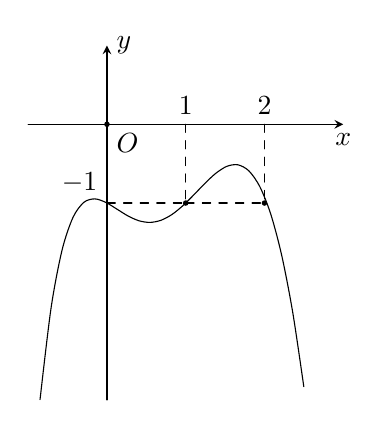
\begin{tikzpicture}[scale=1, line join = round, line cap = round,>=stealth]
	\tikzset{label style/.style={font=\footnotesize}}
	\draw[->] (-1,0) --(0,0) node[below right]{$ O $} --(3,0)node[below]{$ x $};
	\draw[->](0,-3.5)--(0,1)node[right]{$ y $};
	\draw[domain=-.85:2.5,smooth=1000]
	plot(\x,{0.16*(\x)^(5)-1.31*(\x)^(4)+2.56*(\x)^(3)-0.87*(\x)^(2)-0.54*(\x)^(1)-1});
	\draw[dashed] (0,-1)node[above left]{$ -1 $}--(1,-1)--(1,0)node[above]{$ 1 $} (1,-1)--(2,-1)--(2,0)node[above]{$ 2 $};
	\fill[black]circle(1pt)(1,-1)circle(1pt)(2,-1)circle(1pt);
	\end{tikzpicture}
	}
	\loigiai{Xét hàm số $ g(x)=f(x)+x $ có $ g^\prime (x)=f^\prime (x)+1 $.\\ 
	Dựa vào đồ thị hàm số $ y=f^\prime (x) $ có
	$ g^\prime (x)=0\Leftrightarrow f^\prime (x)=-1\Leftrightarrow \hoac{
	& x=0 \\
	& x=1 \\
	& x=2.
	} $ \\
	Bảng biến thiên
	\begin{center}
	\begin{tikzpicture}[>=stealth]
	\tkzTabInit[nocadre,lgt=1.2,espcl=2.5]
	{$ x $ /.6, $ g' $ /.6, $ g $ /2}
	{$ -\infty $, $ 0 $, $ 1 $, $ 2 $, $ +\infty $}
	\tkzTabLine{,-,0,-,0,+,0,-,}
	\node[shift={(0,-.2)}] (A) at (N12) {};
	%	\node[shift={(0,.2)}] (B) at (N23) {$ -4 $};
	\node[shift={(0,-1.5)}] (C) at (N32) {$ \text{CT} $};
	\node[shift={(0,1.5)}] (D) at (N43) {$ \text{CĐ} $};
	\node[shift={(0,-1.5)}] (E) at (N52) {};
	\draw[->,thick] (A)--(C);
	%	\draw[->,thick] (B)--(C);
	\draw[->,thick] (C)--(D);
	\draw[->,thick] (D)--(E);
	\end{tikzpicture}
	\end{center}
	Từ đó suy ra hàm số $ y=g(x) $ đạt cực tiểu tại điểm $ x=1 $.\\	
	}
\end{ex}
%%%=========HetCau_42=========%%%
%%%=========Cau_43=========%%%
\begin{ex}%[2H1B3-2]
	Thể tích $ V $ của khối hộp chữ nhật $ ABCD. A'B'C'D' $ biết $ AB=a, AD=2a, AC'=a\sqrt{14} $ là
	\choice
	{$ V=2a^3 $}
	{$ V=a^3\sqrt{5} $}
	{\True $ V=6a^3 $}
	{$ V=\dfrac{a^3\sqrt{14}}{3} $}
	\loigiai{
	\immini{
	Xét hình chữ nhật ABCD, ta có\\ $ AC^2=AB^2+AD^2=a^2+4a^2=5a^2 $.\\
	Xét tam giác vuông $ AA'C, $ ta có \\$ AA'^2=AC'^2-AC^2=14a^2-5a^2=9a^2.\\
	\Rightarrow AA'=3a $.\\
	Vậy $ V_{ABCD. A'B'C'D'}=AB\cdot AD\cdot AA'=a\cdot2a\cdot3a=6a^3 $.
	}{%
	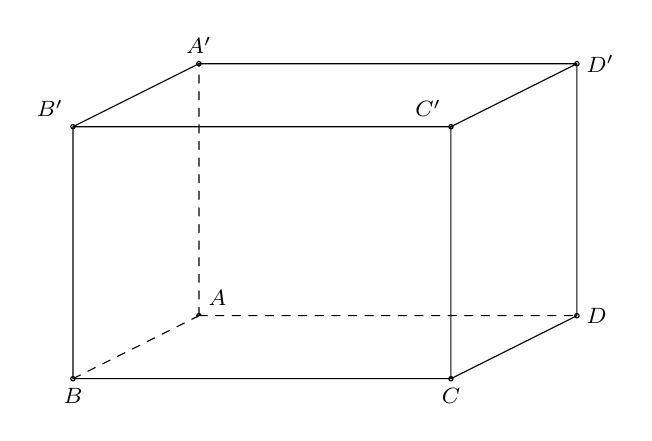
\begin{tikzpicture}[scale=0.8,>=stealth, font=\footnotesize, line join=round, line cap=round]
	\coordinate (B)at(0,0);
	\coordinate (C)at(6,0);
	\coordinate (A)at(2,1);
	\coordinate (D)at(8,1);
	\coordinate (B')at(0,4);
	\coordinate (C')at(6,4);
	\coordinate (A')at(2,5);
	\coordinate (D')at(8,5);
	\draw[] (C)circle(1pt)node[below]{$ C $}--(C')circle(1pt)node[above left]{$ C' $}--(B')circle(1pt)node[above left]{$ B' $}--(B)circle(1pt)node[below]{$ B $}--(C)--(D)circle(1pt)node[right]{$ D $}--(D')circle(1pt)node[right]{$ D' $}--(A')circle(1pt)node[above]{$ A' $}--(B') (C')--(D');	
	\draw[dashed] (B)--(A)circle(1pt)node[above right]{$ A $}--(D) (A)--(A');	
	\end{tikzpicture}
	}
	}
\end{ex}
%%%=========HetCau_43=========%%%
%%%=========Cau_44=========%%%
\begin{ex}%[2H3K3-2]
	Trong không gian với hệ trục $ Oxyz $, đường vuông góc chung của hai đường thẳng chéo nhau $ d_1\colon\dfrac{x-2}{2}=\dfrac{y-3}{3}=\dfrac{z+4}{-5} $ và $ d_2\colon\dfrac{x+1}{3}=\dfrac{y-4}{-2}=\dfrac{z-4}{-1} $ có phương trình là
	\choice
	{$ \dfrac{x-2}{2}=\dfrac{y-2}{3}=\dfrac{z-3}{4} $}
	{\True $ \dfrac{x}{1}=\dfrac{y}{1}=\dfrac{z-1}{1} $}
	{$ \dfrac{x-2}{2}=\dfrac{y+2}{2}=\dfrac{z-3}{2} $}
	{$ \dfrac{x}{2}=\dfrac{y-2}{3}=\dfrac{z-3}{-1} $}
	\loigiai{Giả sử $ AB $ là đoạn vuông góc chung của hai đường thẳng $ d_1 $ và $ d_2 $ với $ A\in d_1 $ và $ B\in d_2 $ \\
	Ta lại có $ A\in d_1\Rightarrow A\left(2+2a;3+3a;-4-5a\right) $ và $ B\in d_2\Rightarrow B\left(-1+3b;4-2b;4-b\right) $.\\
	Ta có $ \overrightarrow{AB}=\left(-3+3b-2a;1-2b-3a;8-b+5a\right) $.\\
	Đường thẳng $ d_1 $ có một véc-tơ chỉ phương $ \overrightarrow{u}_1=\left(2;3;-5\right) $;\\
	$ d_2 $ có một véc-tơ chỉ phương $ \overrightarrow{u}_2=\left(3;-2;-1\right) $.\\
	Vì $ AB $ là đoạn vuông góc chung của $ d_1 $ và $ d_2 $ nên ta có
	$ \heva{
	AB\perp d_1 \\
	AB\perp d_2
	}\Leftrightarrow \heva{
	\overrightarrow{AB}\cdot\overrightarrow{u}_1=0 \\
	\overrightarrow{AB}\cdot\overrightarrow{u}_2=0.
	} $ \\ $ \Leftrightarrow \heva{
	2\left(-3+3b-2a\right)+3\left(1-2b-3a\right)-5\left(8-b+5a\right)=0 \\
	3\left(-3+3b-2a\right)-2\left(1-2b-3a\right)-1\left(8-b+5a\right)=0
	} $ 
	$ \Leftrightarrow \heva{
	-38a+5b=43 \\
	-5a+14b=19
	} $ $ \Leftrightarrow \heva{
	a=-1 \\
	b=1.
	} $ \\ Do đó $ A\left(0;0;1\right) $ và $ \overrightarrow{AB}=\left(2;2;2\right) $ là một véc-tơ chỉ phương của $ AB $, suy ra $ AB $ cũng có một véc-tơ chỉ phương $ \overrightarrow{u}=\dfrac{1}{2}\overrightarrow{AB}=\left(1;1;1\right) $.\\
	Đường thẳng $ AB $ có phương trình chính tắc là $ \dfrac{x}{1}=\dfrac{y}{1}=\dfrac{z-1}{1} $.
	}
\end{ex}
%%%=========HetCau_44=========%%%
%%%=========Cau_45=========%%%
\begin{ex}%[2D2G5-5]
	Số giá trị nguyên dương của tham số $ m $ để bất phương trình $$9^{\sqrt{x^2-3x+m}}+2.3^{\sqrt{x^2-3x+m}-2+x}<3^{2x-3} $$ có nghiệm là
	\choice
	{$ 8 $}
	{\True $ 1 $}
	{$ 6 $}
	{$ 4 $}
	\loigiai{Đặt $ t=3^{\sqrt{x^2-3x+m}-x} $ với $ t>0 $, bất phương trình đã cho trở thành $$ t^2+\dfrac{2}{9}t-\dfrac{1}{27}<0\Leftrightarrow -\dfrac{1}{3}<t<\dfrac{1}{9}.$$
	Do đó $ 0<t<\dfrac{1}{9}\Leftrightarrow \sqrt{x^2-3x+m}-x<-2\Leftrightarrow \sqrt{x^2-3x+m}<x-2 $ \\. 
	$$ \Leftrightarrow \heva{
	& x>2 \\
	& x^2-3x+m\ge 0 \\
	& x^2-3x+m<x^2-4x+4
	} \Leftrightarrow \heva{
	& x>2 \\
	& x^2-3x+m\ge 0 \\
	& x<4-m.
	} \quad (I)$$
	Để bất phương trình đề bài cho có nghiệm thì hệ bất phương trình (I) có nghiệm.\\
	Ta đặt
	$ \heva{
	&x>2& (1)\\
	&x^2-3x+m\ge 0& (2)\\
	&x<4-m & (3).
	} $\\
	Điều kiện cần: Từ $ (1) $ và $ (3) $ ta có $ 4-m>2\Leftrightarrow m<2 $.\\
	Do $ m $ là số nguyên dương nên $ m=1 $.\\
	Điều kiện đủ: Với $ m=1 $, hệ bất phương trình (I) trở thành\\ 
	$$ \heva{
	& x>2 \\
	& x^2-3x+1\ge 0 \\
	& x<3
	} 
	\Leftrightarrow \heva{
	& 2<x<3 \\
	& x<\dfrac{3-\sqrt{5}}{2}\vee x>\dfrac{3+\sqrt{5}}{2}
	} \Leftrightarrow \dfrac{3+\sqrt{5}}{2}<x<3 .$$\\ Vậy hệ bất phương trình (I) có nghiệm.
	}
\end{ex}
%%%%=========HetCau_45=========%%%
%%%=========Cau_46=========%%%
\begin{ex}%[2D3G3-2]
	\immini{
	Bồn hoa của một trường X có dạng hình tròn bán kính bằng $ 8m $. Người ta chia bồn hoa thành các phần như hình vẽ dưới đây và có ý định trồng hoa như sau: Phần diện tích bên trong hình vuông $ ABCD $ để trồng hoa. Phần diện tích kéo dài từ $4$ cạnh của hình vuông đến đường tròn dùng để trồng cỏ. Ở $4$ góc còn lại mỗi góc trồng một cây cọ. Biết $ AB=4m $, giá trồng hoa là $ 200.000 $ đồng$/ m^{2}$, giá trồng cỏ là $ 100.000 $ đồng$/m^{2}$, mỗi cây cọ giá $ 150.000 $ đồng. hỏi cần bao nhiêu tiền để thực hiện việc trang trí bồn hoa đó.
	\choice
	{$ 14.465.000 $ đồng}
	{$ 14.865.000 $ đồng}
	{\True $ 13.265.000 $ đồng}
	{$ 12.218.000 $ đồng}
	}{%
	\begin{tikzpicture}[>=stealth, line join=round, line cap=round, font=\footnotesize, scale=0.8]
	\def\r{3}
	\def\k{.5}
	\draw[pattern=north east lines,pattern color=gray] (0,0) circle(\r);
	\foreach \i/\p in {0/B,1/A,2/D,3/C}{
	\draw[fill=white,rotate=\i*90](30:\r)arc(30:60:\r)|-(30:\r);
	\fill[rotate=\i*90,black!20] (0,0) rectangle (\r/2,\r/2);
	\draw[fill=black,rotate=\i*90]
	(\r/2,\r/2)circle(1pt)+(30:.2)node[scale=.9]{\p};
	}
	\fill[black](0,0)circle(1pt)node[below left,black]{$O$};
	\end{tikzpicture}
	}
	\loigiai{
	\immini{
	Chọn hệ trục tọa độ sao cho gốc tọa độ trùng với tâm hình tròn, suy ra phương trình
	đường tròn là $ x^2+y^2=64 $.\\
	Diện tích hình vuông $ ABCD $ là\\ $ S_{ABCD}=4\times 4=16\left(m^2\right) $.\\
	$ \Rightarrow $ Số tiền để trồng hoa là $$ T_1=16\times 200.000=3.200.000 .$$
	Diện tích trồng cỏ là $$ S=4\displaystyle\int\limits_{-2}^2\left(\sqrt{64-x^2}-2\right) \mathrm{\,d}x\approx 94,654\left(m^2\right) .$$
	$ \Rightarrow $ Số tiền trồng cỏ là $$ T_2=94,654\times 100.000=9.465.000 .$$
	Số tiền trồng 4 cây cọ là $ T_3=150.000\times 4=600.000 $.\\
	Vậy tổng số tiền để thực hiện việc trang trí bồn hoa là
	$$ T=T_1+T_2+T_3=13.265.000 .$$
	}{%
	\begin{tikzpicture}[>=stealth, line join=round, line cap=round, font=\footnotesize, scale=0.8]
	\def\r{3}
	\def\k{.5}
	\draw[pattern=north east lines,pattern color=gray] (0,0) circle(\r);
	\foreach \i/\p in {0/B,1/A,2/D,3/C}{
	\draw[fill=white,rotate=\i*90](30:\r)arc(30:60:\r)|-(30:\r);
	\fill[rotate=\i*90,black] (0,0) rectangle (\r/2,\r/2);
	\draw[fill=black,rotate=\i*90]
	(\r/2,\r/2)circle(1pt)+(30:.2)node[scale=.9]{\p};
	}
	%\draw (0,0)circle(1pt)node[below left]{$ O $};
	\draw[->] (180:\r+\k)--(0:\r+\k)node[below]{$ x $};
	\draw[->] (-90:\r+\k)--(90:\r+\k)node[right]{$ y $};
	\end{tikzpicture}
	}
	}
\end{ex}
%%%=========HetCau_46=========%%%
%%%=========Cau_47=========%%%
\begin{ex}%[2D4G5-1]
	Cho $ z_1, z_2 $ là hai trong các số phức thỏa mãn $ \left| z-3+\sqrt{3}i \right|=2 $ và $ \left| z_1-z_2 \right|=4 $. Giá trị lớn nhất của $ \left| z_1 \right|+\left| z_2 \right| $ bằng
	\choice
	{$ 2+2\sqrt{3} $}
	{$ 4\sqrt{3} $}
	{$ 4 $}
	{\True $ 8 $}
	\loigiai{
	\immini{ Gọi $ M, N $ lần lượt là điểm biểu diễn của hai số phức $ z_1, z_2 $.\\
	Do $ \heva{
	& \left| z_1-3+\sqrt{3}i \right|=\left| z_2-3+\sqrt{3}i \right|=2 \\
	& \left| z_1-z_2 \right|=4
	} $\\ nên $ \heva{
	& M,N\in (C)\colon \left(x-3\right)^2+\left(y+\sqrt{3}\right)^2=2^2 \\
	& MN=4=2\cdot2.
	} $ 
	}{%
	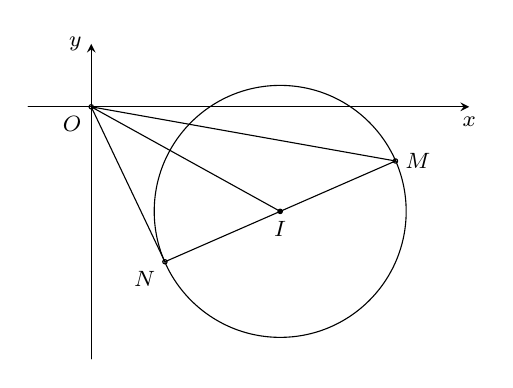
\begin{tikzpicture}[scale=0.8,>=stealth, font=\footnotesize, line join=round, line cap=round]
	\def\xmin{-1}\def\xmax{6}\def\ymin{-4}\def\ymax{1} 
	\draw[->] (\xmin,0)--(\xmax,0) node [below]{$ x $};
	\draw[->] (0,\ymin)--(0,\ymax) node [left]{$ y $};
	\draw (3,-1.66)node[below]{$ I $}circle(2) (0,0)circle (1pt)node[below left]{$ O $} (1.17,-2.46)circle (1pt)node[below left]{$ N $} (4.83,-0.86)circle(1pt)node[right]{$ M $}; \draw[fill=black](3,-1.66)circle(1pt);
	\draw (0,0)--(1.17,-2.46)--(4.83,-0.86)--(0,0)--(3,-1.66);	
	\end{tikzpicture}
	}
	\noindent
	Như vậy $ MN $ là đường kính của đường tròn $ (C) $ với tâm $ I\left(3;-\sqrt{3}\right) $, bán kính $ R=2 $, do đó $ I $ là trung điểm $ MN $, $ \mathrm{O}I=\sqrt{12} $.\\
	Ta có $ \left| z_1 \right|+\left| z_2 \right|=OM+ON \le \sqrt{\left(1+1\right)\left(OM^2+ON^2\right)}=\sqrt{2\left(2\mathrm{O}I^2+\dfrac{MN^2}{2}\right)}=8 $.\\
	Dấu $\lq\lq =\lq\lq $ xảy ra khi và chỉ khi $ OM=ON\Leftrightarrow MN $ là đường kính của $ (C) $ vuông góc với $ OI $.
	}
\end{ex}
%%%=========HetCau_47=========%%%
%%%=========Cau_48=========%%%
\begin{ex}%[2H3G2-7]%[2H3G2-8]
	Trong không gian $ Oxyz $, cho hình nón có đỉnh $ I $ thuộc mặt phẳng $ (P)\colon 2x-y-2z-7=0 $ và hình tròn đáy nằm trên mặt phẳng $ (R)\colon 2x-y-2z+8=0 $. Mặt phẳng $ (Q) $ đi qua điểm $ A\left(0;-2;0\right) $ và vuông góc với trục của hình nón chia hình nón thành hai phần có thể tích lần lượt là $ V_1 $ và $ V_2 $ ($ V_1 $ là thể tích của hình nón chứa đỉnh $ I $). Biết bằng biểu thức $ S=V_2+\dfrac{78}{V_1^3} $ đạt giá trị nhỏ nhất khi $ V_1=a $, $ V_2=b $. Khi đó tổng $ a^2+b^2 $ bằng
	\choice
	{$ 52\sqrt{3}\pi^2 $}
	{$ 377\sqrt{3} $}
	{\True $ 2031 $}
	{$ 2031\pi^2 $}
	\loigiai{
	\immini{Dễ thấy $ (P) \parallel (R) $, gọi $ O $ là tâm của đường tròn đáy hình nón, $ O'=IO\cap (Q) $, từ giả thiết ta có
	$ IO'=\mathrm{d}\left(A,(P)\right)=\dfrac{5}{3} $; $ OO'=\mathrm{d}\left(A,(R)\right)=\dfrac{10}{3} $ suy ra $ OO'=2IO' $.\\
	Gọi $ M $ là điểm thuộc đường tròn $ (O) $, $ M'=IM\cap (Q) $, do $ O'M' \parallel OM $ nên $ \dfrac{IO'}{IO}=\dfrac{O'M'}{OM}=\dfrac{1}{3} $.\\
	Do đó $ r_2=3r_1 $, (trong đó $ r_1 $ và $ r_2 $ lần lượt là bán kính của các đường tròn $ \left(O'\right) $ và $ (O) $).\\ 
	Đặt $ IO'=h $, khi đó
	$ \dfrac{V_1}{V}=\dfrac{\dfrac{1}{3}\pi r_1^2h}{\dfrac{1}{3}\pi{\left(3r_1\right)^2}\cdot 3h}=\dfrac{1}{27} $ \\ $ \Rightarrow V=27V_1\Rightarrow V_2=V-V_1=26V_1 $.\\
	}{%
	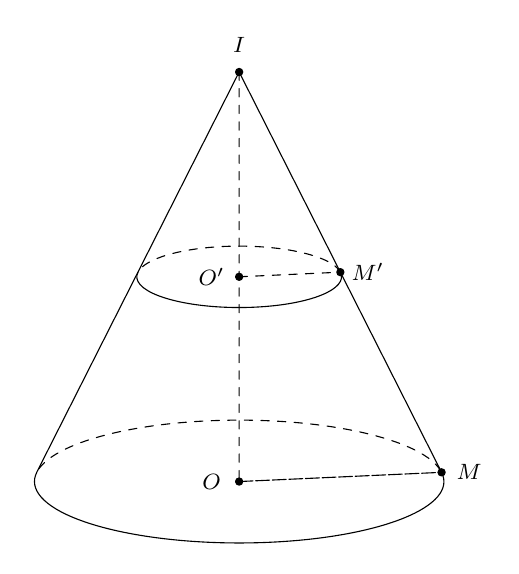
\begin{tikzpicture}[font=\footnotesize, line join=round,scale=1.3, line cap=round, >=stealth]
	\def\h{4}
	\def\l{0.5*\h}
	\def\a{2}
	\def\b{0.3*\a}
	\pgfmathsetmacro{\t}{asin(\b/\h)}
	\begin{scope}
	\path(\t:{\a} and {\b})coordinate(M) arc(\t:180-\t:{\a} and {\b})coordinate(N)(0,\h)coordinate(I)(0,0)coordinate(O);
	\draw(N)--(I)--(M)(M) arc(\t:-180-\t:{\a} and {\b})coordinate(N);
	\end{scope}
	\begin{scope}[shift={(0,\l)},scale=0.5]
	\path(\t:{\a} and {\b})coordinate(M')(0,0)coordinate(O');
	\draw(M') arc(\t:-180-\t:{\a} and {\b})coordinate(N);
	\draw[dashed](M')arc(\t:180-\t:{\a} and {\b});
	\end{scope}
	\draw[dashed](I)--(O)--(M)arc(\t:180-\t:{\a} and {\b})(O')--(M')(O)--(M);
	\foreach \d/\g in{I/90,M/0,O/180,O'/180,M'/0}
	\draw[fill=black](\d)circle(1pt)node[shift={(\g:0.35)}]{$\d$};
	\end{tikzpicture}
	}
	\noindent
	$ S=V_2+\dfrac{78}{V_1^3}=26V_1+\dfrac{78}{V_1^3}=\dfrac{26}{3}V_1+\dfrac{26}{3}V_1+\dfrac{26}{3}V_1+\dfrac{78}{V_1^3}\ge 4\sqrt[4]{\dfrac{26}{3}V_1\cdot\dfrac{26}{3}V_1\cdot \dfrac{26}{3}V_1\cdot\dfrac{78}{V_1^3}}=4\sqrt[4]{\dfrac{456976}{9}} $.\\
	Dấu  \lq\lq=\rq\rq\  xảy ra khi $ \dfrac{26}{3}V_1=\dfrac{78}{V_1^3}\Leftrightarrow V_1=\sqrt{3} $.\\
	Suy ra $ \heva{
	& a=\sqrt{3}\\
	& b=26\sqrt{3}.
	} $ \\
	Vậy $ a^2+b^2=3+26^2\cdot3=2031 $.
	}
\end{ex}
%%%=========HetCau_48=========%%%
%%%=========Cau_49=========%%%
\begin{ex}%[2D1G2-2]
	\immini{
	Cho đồ thị hàm số $ y=f(x) $ như hình vẽ bên
	Số điểm cực đại, cực tiểu của hàm số $ g(x)=\left[f(x) \right]^2 $ là
	\motcot
	{$1$ điểm cực đại, $3$ điểm cực tiểu}
	{$3$ điểm cực đại, $2$ điểm cực tiểu}
	{$2$ điểm cực đại, $2$ điểm cực tiểu}
	{\True $2$ điểm cực đại, $3$ điểm cực tiểu}
	}{%
	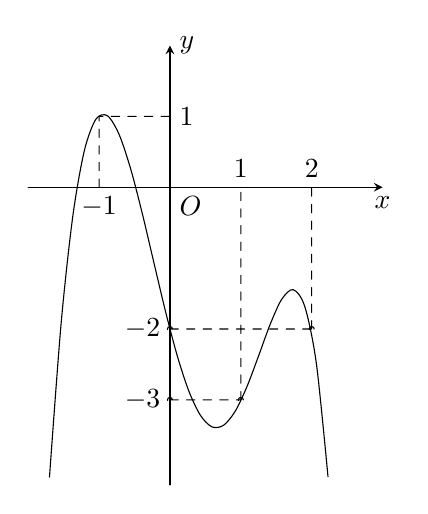
\begin{tikzpicture}[scale=0.9, line join = round, line cap = round,>=stealth]
	\tikzset{label style/.style={font=\footnotesize}}
	\draw[->] (-2,0) --(0,0) node[below right]{$ O $} --(3,0)node[below]{$ x $};
	\draw[->](0,-4.2)--(0,2)node[right]{$ y $};
	\draw[domain=-1.7:2.23,smooth=300]
	plot(\x,{-0.13*(\x)^(5)-0.67*(\x)^(4)+1.98*(\x)^(3)+1.67*(\x)^(2)-3.86*(\x)^(1)-2});
	\draw[dashed](-1,0)node[below]{$ -1 $}--(-1,1)--(0,1)node[right]{$ 1 $} (0,-2)circle(1pt)node[left]{$ -2 $} (0,-3)circle(1pt)node[left]{$ -3 $} (0,-3)--(1,-3)circle(1pt)--(1,0)node[above]{$ 1 $} (0,-2)--(2,-2)circle(1pt)--(2,0)node[above]{$ 2 $};	
	\end{tikzpicture}
	}
	\loigiai{Ta có $ g'(x)=2f(x)\cdot f'(x) $. Suy ra $ g'(x)=0\Leftrightarrow \hoac{
	& f(x)=0~ (1) \\
	& f'(x)=0~ (2).
	} $ \\
	Pt (1) $ \Leftrightarrow \hoac{
	& x=a \in \left(-\infty;-1\right) \\
	& x=b \in \left(-1;0\right).
	} $\\
	Pt (2) $ \Leftrightarrow \hoac{
	& x=x_1\in \left(-1;b\right) \\
	& x=x_2\in \left(0;1\right) \\
	& x=x_3\in \left(1;2\right)
	} $, trong đó $ x_1,x_3 $ là các điểm cực đại và $ x_2 $ là các điểm cực tiểu.\\
	Bảng biến thiên
	\begin{center}\begin{tikzpicture}[>=stealth]
	\tkzTabInit[nocadre,lgt=1.2,espcl=2.5]
	{$ x $ /.6, $ f'(x) $ /.6, $ f(x) $ /.6, $ g'(x) $ /.6, $ g(x) $ /2}
	{$ -\infty $, $ a $, $ x_1 $, $ b $, $ x_2 $, $ x_3 $, $ +\infty $}
	\tkzTabLine{,+,|,+,0,-,0,-,0,+,0,-,}
	\tkzTabLine{,-,0,+,|,+,0,-,|,-,|,-,}
	\tkzTabLine{,-,0,+,0,-,0,+,0,-,0,+,}
	\node[shift={(0,-1.5)}] (A) at (N12) {$ +\infty $};
	\node[shift={(0,-2)}] (B) at (N23) {$ \text{CT} $};
	\node[shift={(0,-1.5)}] (C) at (N32) {$ \text{CĐ} $};
	\node[shift={(0,-2)}] (D) at (N43) {$ \text{CT} $};
	\node[shift={(0,-1.5)}] (E) at (N52) {$ \text{CĐ} $};
	\node[shift={(0,-2)}] (F) at (N63) {$ \text{CT} $};
	\node[shift={(0,-1.5)}] (G) at (N72) {$ +\infty $};
	\draw[->,thick] (A)--(B);
	\draw[->,thick] (B)--(C);
	\draw[->,thick] (C)--(D);
	\draw[->,thick] (D)--(E);
	\draw[->,thick] (E)--(F);
	\draw[->,thick] (F)--(G);
	\end{tikzpicture}\end{center}
	}
\end{ex}
Từ bảng biến thiên trên suy ra hàm số $ g(x)=\left[f(x) \right]^2 $ có $2$ điểm cực đại, $3$ điểm cực tiểu.\\
%%%=========HetCau_49=========%%%
%%%=========Cau_50=========%%%
\begin{ex}%[2D1G1-4]
	Có bao nhiêu giá trị nguyên của tham số $ m\in \left[-2019;2019 \right] $ để phương trình \break $ 2019^x+\dfrac{2x-1}{x+1}+\dfrac{mx-2m-1}{x-2}=0 $ có đúng $3$ nghiệm thực phân biệt?
	\choice
	{$ 4039 $}
	{$ 4038 $}
	{$ 2019 $}
	{\True $ 2017 $}
	\loigiai{Ta có phương trình\\ $$ 2019^x+\dfrac{2x-1}{x+1}+\dfrac{mx-2m-1}{x-2}=0\Leftrightarrow{2019^x}+\dfrac{2x-1}{x+1}+\dfrac{m(x-2)-1}{x-2}=0 $$
	$$ \Leftrightarrow{2019^x}+\dfrac{2x-1}{x+1}+m-\dfrac{1}{x-2}=0\Leftrightarrow m=\dfrac{1}{x-2}-2019^x-\dfrac{2x-1}{x+1} .$$
	Xét hàm số $ y=\dfrac{1}{x-2}-2019^x-\dfrac{2x-1}{x+1}{;}\,x\in \mathbb{R}\setminus \left\{-1;2 \right\}\\
	\Rightarrow y'=-\dfrac{1}{(x-2)^2}-2019^x\ln 	(2019)-\dfrac{3}{(x+1)^2}<0;\forall x\in \mathbb{R}\setminus \left\{-1;2 \right\} $.\\
	Bảng biến thiên
	\begin{center}
\begin{tikzpicture}
	\tkzTabInit[nocadre,lgt=1.2,espcl=2,deltacl=.6]
	{$ x $ /0.6, $ y' $ /0.6, $ y $ /2}
	{$ -\infty $, $ -1 $, $ 2 $, $ +\infty $}
	\tkzTabLine{,-,d,-,d,-,}
	\tkzTabVar{+/ $ -2 $,-D+/ $ -\infty $ / $ +\infty $,-D+/ $ 	-\infty $ / $ +\infty $, -/ $ -\infty $}
	\end{tikzpicture}\end{center}
	\noindent
	Vậy để phương trình có $3$ nghiệm phân biệt thì $ m\in \left(-\infty;-2\right) $ mà $ m\in \left[-2019;2019 \right];m\in \mathbb{Z} $.\\ Vậy ta có $ 2017 $ số nguyên $ m $ cần tìm.\\
	}
\end{ex}
%%%=========HetCau_50=========%%%

\Closesolutionfile{ans}